\documentclass{resume}
\usepackage[colorlinks=True]{hyperref}
\usepackage{xcolor}
\usepackage{multicol}

\usepackage{graphicx}
\usepackage[maxnames=99]{biblatex}
\addbibresource{references.bib}

\usepackage[left=0.75in,top=0.6in,right=0.75in,bottom=0.6in]{geometry} % Document margins
\newcommand{\tab}[1]{\hspace{.2667\textwidth}\rlap{#1}}
\newcommand{\itab}[1]{\hspace{0em}\rlap{#1}}

\name{Sarthak Kapoor}

\begin{document}

\begin{rSection}{Personal Information}\itemsep -3pt
\begin{multicols}{2}

  \begin{tabular}{|ll}
    Address: & Kullenhofstr. 56, Aachen 52074, Germany \\
    Email: & sarthak.kapoor@rwth-aachen.de \\
    Contact: & +49 162 5483728 \\
    Languages: &  English and Hindi (Bilingual proficiency) \\
    Date of birth: &  Nov. 1, 1997 \\ 
    Nationality: &  India \\
    Personal Website: & \url{https://ka-sarthak.github.io/}\\
  \end{tabular}
  \columnbreak
  \hfill 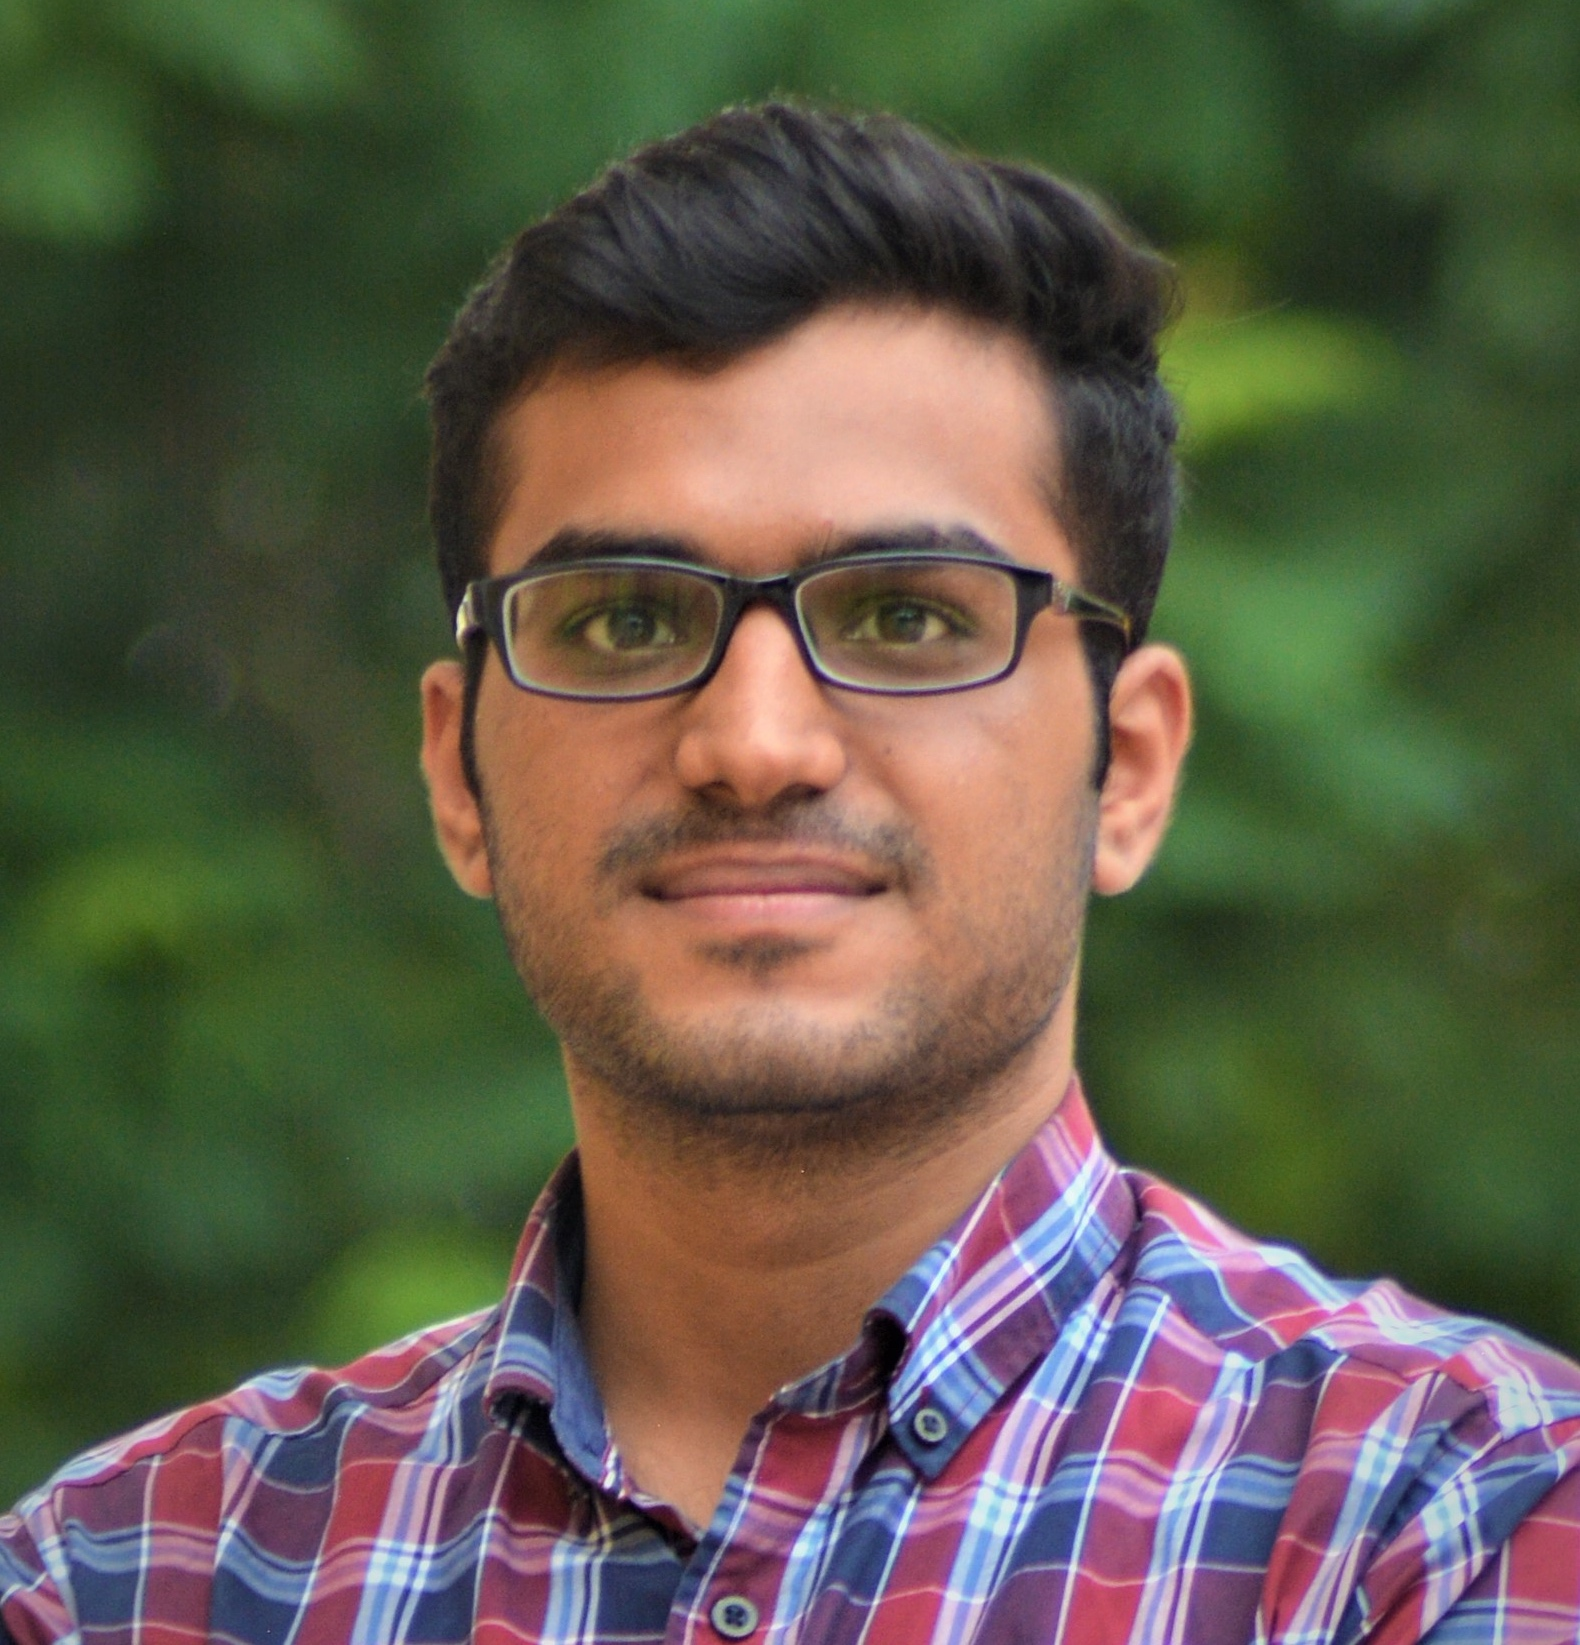
\includegraphics[width=3.5cm]{profile.jpg}

\end{multicols}
\end{rSection}

%\begin{rSection}{Objective}
%Self-motivated master's student seeking experience in the field of %process simulation and optimization and novel applications of Machine %Learning techniques.
%\end{rSection}

\begin{rSection}{Education}
{\bf RWTH Aachen University} \hfill {\em 2020.10 - Present}\\
MSc Simulation Sciences \hfill {CGPA: 2.2}\\
Focus: Applied mathematics, machine learning, computational modeling \hfill{(German scale)}

{\bf Machine Learning Summer School (MLSS\(^N\))} \hfill {\em 2022.06}\\
{\em Jagiellonian University, Poland}\\
Participated with a full scholarship

{\bf National Institute of Technology, Warangal} \hfill {\em 2016.08 - 2020.08} \\
BTech Metallurgical and Materials Engineering\hfill {CGPA: 9.13 (10)}\\
\emph{Gold Medallist}
%{\bf Sacred Heart Convent School, Ludhiana} \hfill {\em 2015.03 - 2016.05}\\
%Grade 12 CBSE (Physics, Chemistry, Mathematics, English) \hfill {Percentage: 95.4 }
%\emph{Batch Rank: 3}
%{\bf DAV Public School, Ludhiana} \hfill {\em 2015.03 - 2016.05}\\
%Grade 10 CBSE \hfill {CGPA: 10}\\
\end{rSection}

\begin{rSection}{Work Experience}
{\bf Wissenschaftliche Hilfskraft (Research Assistant)} \hfill {\em 2021.05 - Present}\\
{\em Chair for Material Mechanics, RWTH Aachen}\\
As a research assistant under Prof. Bob Svendsen, I am developing learning-based approaches to infer solutions of differential equations involved in solid mechanics, thereby providing an alternative to expensive numerical solvers. Working extensively with Python, TensorFlow, PyTorch.

{\bf Application Development Analyst} \hfill {\em 2020.09 - 2020.12}\\
{\em Accenture Technology Center, Bengaluru}\\
During my stint as an Application Development Analyst at Accenture, I learned a great deal about conceptualizing software solutions and trained in software-delivery methods.
\end{rSection}

\begin{rSection}{Projects}
{\bf Detecting gravity waves in atmospheric temperature data} \hfill {\em2022.06}\\
{\em Applied and Computational Mathematics, RWTH Aachen}\\
As part of a week-long study excursion, we developed an algorithm to detect gravity wave events, which are essential for reliable weather predictions, in large datasets of atmospheric temperature. The project was supervised by Dr. Joern Ungermann from Forschungszentrum Jülich and the code was written in Python using NumPy, SciPy, JAX libraries.

{\bf Tracking local optima in dynamic systems}\hfill {\em 2021.10 - 2022.02}\\
{\em Software and Tools for Computational Engineering, RWTH Aachen}\\
Supervised by Prof. Uwe Naumann from Informatik-12, this semester-long project focused on building local-optima-tracking software for dynamic time-dependent functions. The software was written in C++ using dco/c++ library for automatic differentiation. 

{\bf Fast iterative solvers for linear systems}\hfill {\em 2021.04 - 2021.09}\\
{\em Aachen Institute for Advanced Study in Computational Engineering Science, RWTH Aachen}\\
Programmed multigrid solvers, Krylov-based linear system solvers (GMRES and CG) and eigensolver algorithms (Lanczos and Power Iteration) for huge sparse matrices taken from MatrixMarket. These implementations used vanilla Python code without computational libraries.

{\bf Simulation of Mold Filling in LPIM (MITACS Scholar)} \hfill {\em 2019.05 - 2019.08}\\
{\em Ecole Technologie Superieure, Montreal}\\
As a summer research intern, I worked on optimizing LPIM injection stage for metallic feedstock using FEM simulations and experimentation. I also worked on an initial layout of a new viscosity model that accurately captured viscosity behavior for our application. Gained experience in Moldflow, AutoCAD, MATLAB, and feedstock preparation.

{\bf Phase Field Modeling of Ternary System} \hfill {\em 2018.11 - 2019.04}\\
{\em National Institute of Technology, Warangal}\\
During this semester-long bachelor project, I built a simulation routine to study the growth kinetics of precipitates in a hypothetical ternary alloy system. It was based on a phase-field model with semi-implicit spectral formulation and written in C using FFT libraries.
\end{rSection}

\begin{rSection}{Skills}
% \begin{itemize}
  \item \textbf{Development} \textemdash  C/C++, Python (TensorFlow, PyTorch, NumPy, SciPy, JAX, Scikit-Learn, Pandas), MATLAB, Java, OpenMP, MPI, DCO,  HTML, Javascript, MySQL, {\LaTeX}, GitHub.
  \item \textbf{Pursuits} \textemdash Machine Learning (Deep Learning, Neural Networks, Neural Operators, Computer Vision, Data Analytics), Phase-field modeling, Continuum modeling, Automatic Differentiation, Parallel Computing, Fast Iterative Solvers
% \end{itemize}
\end{rSection}

\begin{rSection}{Communication}
Poster presented at MLSS 2022 \textemdash``Correlative modeling of microstructure and stress in solid mechanics using Machine Learning"

Published article \textemdash\fullcite{Cote2021}

\end{rSection}


\begin{rSection}{Volunteering}
{\bf Project Aakaar: Making geometry accessible to visually impaired}\hfill {\em 2019.01 - Present}\\
Started as a bachelor's project at the maker space of NIT Warangal, Project Aakaar has expanded into a global network of designers, thinkers, managers, and engineers, with the common goal of making technical education accessible in the special schools of developing countries like India.
\end{rSection}

\begin{rSection}{Awards} \itemsep -3pt
\item Recipient of a full scholarship to attend Machine Learning Summer School 2022 in Krakow, Poland
\item Recipient of Late Pendyala Upendra Gold Medal 2020 for academic excellence in BTech degree
% \item Honored by Indian Institute of Metals, Hyderabad chapter, for academic excellence in BTech degree
\item Recipient of MITACS 2019 scholarship to pursue research at ETS Montreal \hfill 
\item Recipient of NIT Warangal Merit Scholarship 2016, 2017, 2018, 2019 (Full Tuition Award)
\item Recipient of the prestigious OPJEMS award for two consecutive years 2018, 2019 \hfill 
% \item Recipient of Central Scheme National Scholarship 2016, 2017, 2018 \hfill 


\end{rSection}
\end{document}
